% Remplacer les apostrophes ’ par des quotes '

\begin{frame}{\fe{Exercice 2 : fissuration par suppression d'éléments}
                 {Exercise 2: fracture by elements removal}}
             {\fe{Solution (bis) avec PERSO1}{Solution (bis) with PERSO1}}
  \footnotesize
  \begin{itemize}
    \item \fe{Utiliser la procédure \kwv{PERSO1}}{Use procedure \kwv{PERSO1}}
    \item \fe{Extraire le modèle et les contraintes dans \kwg{'ESTIMATION'}}{Extract the model and stress field in \kwg{'ESTIMATION'}}
    \item \fe{Calculer la contrainte principale $\sigma_I$}{Compute the 1st principal stress $\sigma_I$}
    \item \fe{Extraire les éléments "intacts"}{Extract the "intact" elements}
    \item \fe{Réduire les \g{\red{blocages}} sur ce maillage} et écraser \kwg{'WTABLE'.'BLOCAGES\_MECANIQUES'}
             {Reduce the \g{\red{boundary conditions}} on this mesh and overwrite \kwg{'WTABLE'.'BLOCAGES\_MECANIQUES'}}
    \item \fe{Réduire les pas de temps}{Reduce time steps}
    \item \fe{Activer l'option \kwg{'GRANDS\_DEPLACEMENTS'}}{Use option \kwg{'GRANDS\_DEPLACEMENTS'}}
  \end{itemize}
  \vspace{4.5cm}
  \scriptsize
  \begin{textblock*}{10cm}(0.3cm,-3.2cm)
    \fe{\emph{Programme principal}}{\emph{Main program}}
    \lstinputlisting[basicstyle=\ttfamily\tiny, language=gibiane, firstline=92, lastline=95]{dgibi/formation_pasapas_2_solution_bis.dgibi}
  \end{textblock*}
  \begin{textblock*}{10cm}(6.2cm,-4cm)
    \fe{\emph{\violet{Procédure PERSO1}}}{\emph{\violet{PERSO1 procedure}}}
    \lstinputlisting[basicstyle=\ttfamily\tiny, language=gibiane, firstline=75, lastline=84]{dgibi/formation_pasapas_2_solution_bis.dgibi}
  \end{textblock*}
\end{frame}

\begin{frame}{\fe{Exercice 2 : fissuration par suppression d'éléments}
                 {Exercise 2: fracture by elements removal}}
             {\fe{Solution (bis) avec PERSO1}{Solution (bis) with PERSO1}}
  \footnotesize
  \begin{itemize}
    \item \fe{Résultats}{Results}
    \vspace{0.2cm}
    \begin{center}
      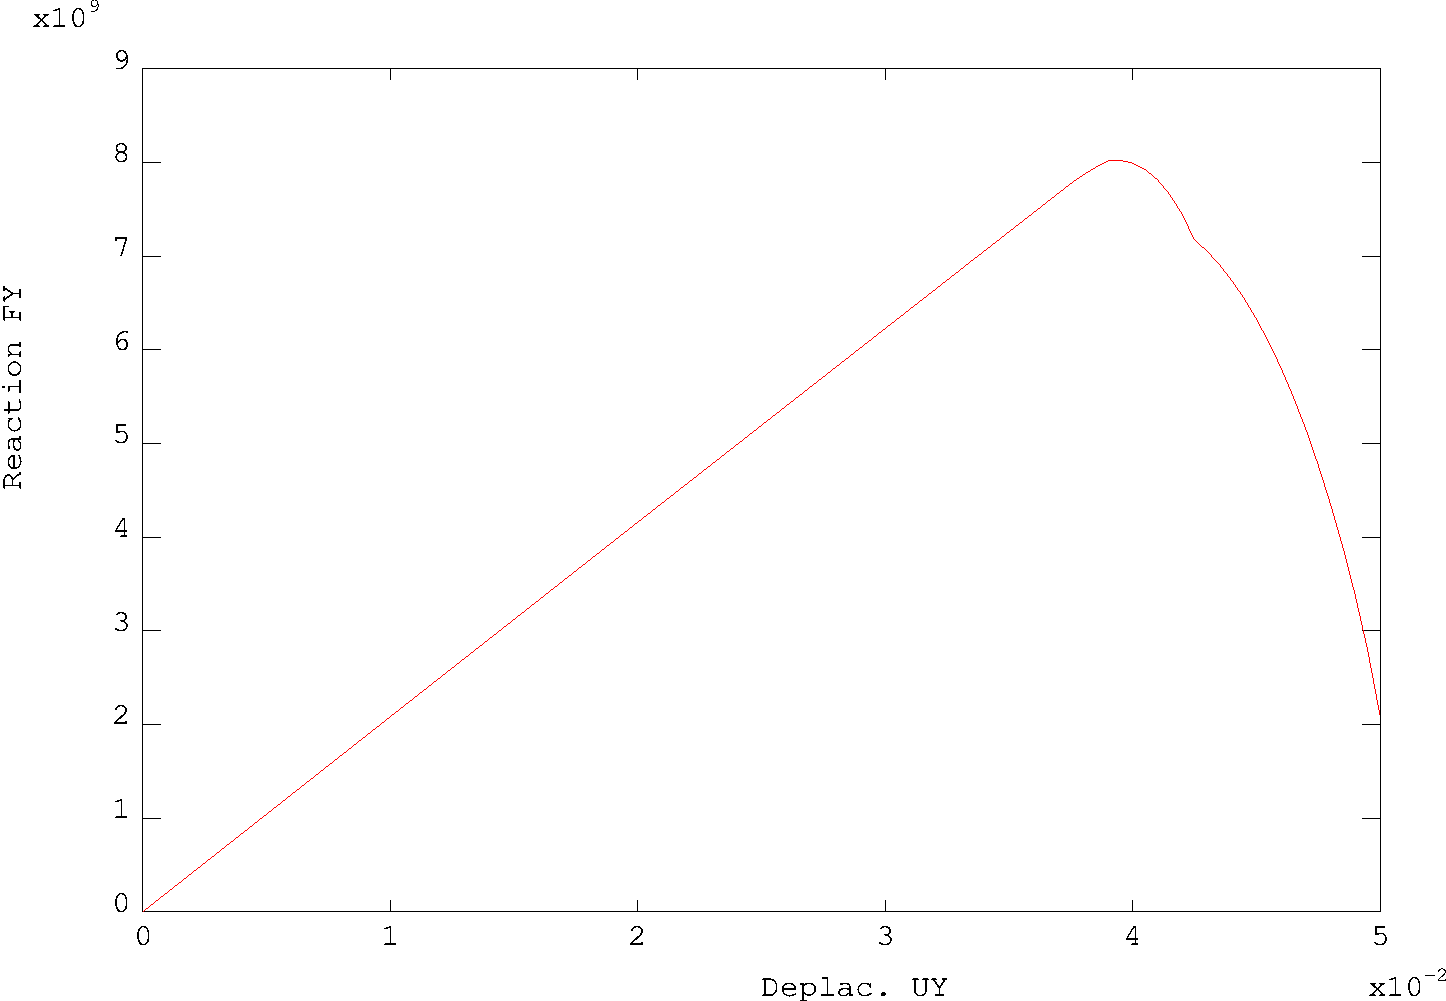
\includegraphics[height=3.5cm]{images/exo/exo_2_solu_bis_evol}
      \hspace{0.4cm}
      \animategraphics[controls,loop,poster=last,height=3.5cm]{10}{images/exo/exo_2_solu_bis_sigma.}{01}{46}
    \end{center}
    \item \fe{Modèle peu robuste\\ résultats très sensibles à la discrétisation espace/temps}
             {Undependable model\\ results quite sensitive to time/space discretization}
  \end{itemize}
\end{frame}
